\section{Motivation for Cohomology}
One of the most important invariants of schemes is \'etale cohomology.  Cohomology is an important invariant in geometry and topology which associates to each space $X$ a sequence of abelian groups $H^i(X)$, $i \ge 0$, the cohomology groups of $X$. For each map $f: X \to Y$ of spaces there are homomorphisms $f^*: H^i(Y) \to H^i(X)$. Moreover there are so called coboundary morphisms $\partial^i : H^i \to H^{i+1}$ for each $i \ge 0$.
\begin{definition}
	A \textit{cohomology theory} for
\end{definition}
We can deduce many interesting properties of spaces from their cohomology groups and the associated homomorphisms.

An important and intuitive cohomology is \textit{singular cohomology}. It provides a rigorous way for counting ``holes'' in a topological space. For instance, the circle $S^1$ has 1 one-dimensional hole while the torus $T^2$ has 2. The sphere $S^2$ has 1 two-dimensional hole but no one-dimensional holes, in symbols\footnote{$\Z$ appears here because it is the free group on one generator.}
\begin{align*}
	H^1_{sing}(S^1) \simeq \Z,\quad & H^1_{sing}(T^2) \simeq \Z \oplus \Z, \\
	H^1_{sing}(S^2) \simeq  0,\quad & H^2_{sing}(S^2) \simeq \Z.
\end{align*}
A general approach to cohomology is to use sheaves on a topological space as ``coefficients''. Sheaves consist of local data on a space that is glueable. A basic example consists of functions on a space: If we have an open cover $\{ U_i\}$ for a manifold $M$ and functions $f_i: M \to \R$ that agree on all intersections $U_i \cap U_j$ we may patch it together to a function $f: M \to \R$.
For any space $X$ and any sheaf $\Sh{F}$ on $X$ we can define $H^i(X, \Sh{F})$. Many examples of cohomology theories turn out to stem from the cohomology of a particular sheaf. For example, if $X$ is a locally contractible space, the singular cohomology $H_{\text{sing}}^i(X)$ of $X$ is isomorphic to the sheaf cohomology $H^i(X, \Z_X)$ of the constant sheaf $\Z_X$ on $X$.

One of the main motivations for \'etale cohomology is that one would like a replacment for singular cohomology for schemes. There are a number of obstacles:
\begin{proposition}\label{scheme_contractible}
	An irreducible scheme is contractible.
\end{proposition}
\begin{proof}
	Define a map $f: X \times I \to X$  by $f(x,0) = x$ and $f(x,t) = \eta$ for $t > 0$. This is a contraction of $X$ onto the point $\eta$, so the singular cohomology of $X$ is identically 0.
\end{proof}

\begin{proposition}
	$H^i(X, \Sh{F})$ is 0 for any sheaf on an irreducible topological space.
\end{proposition}
\begin{proof}
	See section TODO.
\end{proof}
This is a strong indication that the traditional tools of cohomology are inadequate to analyse the geometry of schemes.

\subsection{Exact sequences and Cohomology}

In linear algebra the notions of kernel and cokernel quantify the failure of a map to be injective or surjective. If a map has trivial kernel, it is injectve, if it has trivial cokernel, it is surjective. Cohomology plays a similar role in homological algebra, where we are often faced with the following situation:
Let
\[
	0 \to A \to B \to C \to 0
\]
be an exact sequence in an abelian category $C$ and $F$ a left exact functor to abelian groups. This means that
\[
	0 \to F(A) \to F(B) \to F(C)
\]
is exact. We  would like to fill in this exact sequence on the right with functors $H^i(-): C \to \Ab$ for $i \ge 0$ with the following properties:
\begin{enumerate}
	\item The cohomology $H^0(A)$ in degree 0 should be $F(A)$
	\item Given a short exact sequence as above, there should be a long exact sequence
	      \[
		      \cdots H^i(A) \shortto H^i(B) \shortto H^i(C) \shortto H^{i+1}(A) \shortto H^{i+1}(B) \shortto H^{i+1}(C) \shortto \cdots
	      \]
\end{enumerate}

We have seen that both the global sections functor $\Gamma(X,-): \Ab(X) \to \Set$ and the fixed-point functor left exact. The theory of derived functors allows us to define cohomology for left (or right) exact functors quite generally, as long as the domain of the functor has enough injectives. An injective object $I$ is one for which the functor $\Hom(-,I)$ is exact. If $C$ is an abelian category with enough injectives, every object $A$ has an injective resolution $A \to I^\bullet$, which is an exact sequence
\[
	0 \to A \to I^0 \to I^1 \to \cdots
\]
where each $I^k$ is an injective object. Given a left exact functor $F$ from $C$ to some other abelian category (in our case abelian groups), one defines the $i$-th right derived functor $R^i F$ by choosing for each object $A$ of $C$ an injective resolution $A \to I^\bullet$ and defining
\[
	R^i F(A) \coloneqq H^i(F(I^\bullet)).
\]
One needs to show that these functors do not depend on the choice of injective resolution. While very general, the formalism of derived functors is unintuitive and in practice we will compute cohomology using different methods.

Another functor whose derived functors are of interest is the direct image functor.

\subsection{Homological algebra in \texorpdfstring{$\mathsf{Ab}(X)$}{Ab(X)}}

We will now define the notion of injectivity and surjectivity for maps of sheaves. The categorification of injective mpas are monomorphisms, while surjective maps correspond to epimorphisms. Epimorphisms of sheaves are tricky and the reason why sheaf cohomology is a non-trivial invariant. The general frameworks in which to study (co-)homology are abelian categories. The notion of an abelian category is an abstraction of the category of abelian groups. Abelian categories are the general setting in which to do homological algebra.

\begin{definition}[Monomorphisms and Epimorphisms]
	Let $f: X \to Y$ be a morphism (in any category). We say that $f$ is a \textit{monomorphism} if $f \circ g_1 = f \circ g_2 \implies g_1 = g_2$.
	We say that $f$ is a \textit{epimorphism} if $g_1 \circ  f  = g_2 \circ f \implies g_1 = g_2$.
\end{definition}

\begin{proposition}[Monomorphisms in $\sh(C,J)$]
	Let $\varphi: F \to G$ be a morphism of sheaves on a site $(C,J)$. We say that $\varphi$ is injective if for each object $U$ of $C$, the map $\varphi: F(U) \to G(U)$ is injective.
\end{proposition}

\begin{proposition}[Epimorphisms in $\sh(C,J)$]
	A morphism of sheaves $\varphi: F \to G$ is an epimorphism in $\Sh(C,J)$ if and only if for every object $U$ and every section $s \in G(U)$ there exists a covering $\{U_i \to U\}$ such that the restriction $s|_{U_i}$ is contained in the image of $\varphi: F(U_i) \to G(U_i)$. We also say that \textit{$\varphi$ is locally surjective}.
\end{proposition}

\begin{proof}
	$\implies:$ Suppose that $\varphi$ is locally surjective. For any object $U$ of $C$ and any $s \in G(U)$ choose a cover $\{f_i: U_i \to U\}$ as stated in the proposition. Let $\alpha_1, \alpha_2: G \to H$ be morphisms such that $\alpha_1 \circ \varphi = \alpha_2 \circ \varphi$.
	\[
		% https://q.uiver.app/?q=WzAsMyxbMCwwLCJGIl0sWzEsMCwiRyJdLFsyLDAsIkgiXSxbMCwxLCJcXHZhcnBoaSJdLFsxLDIsIlxcYWxwaGFfMiIsMix7Im9mZnNldCI6MX1dLFsxLDIsIlxcYWxwaGFfMSIsMCx7Im9mZnNldCI6LTF9XV0=
		\begin{tikzcd}
			F & G & H
			\arrow["\varphi", from=1-1, to=1-2]
			\arrow["{\alpha_2}"', shift right=1, from=1-2, to=1-3]
			\arrow["{\alpha_1}", shift left=1, from=1-2, to=1-3]
		\end{tikzcd}\]
	We need to show that $\alpha_1 = \alpha_2$.  Now for each $f_i: U_i \to U$ and each section $s \in F(U)$ we have $(\alpha_1 \circ f_i)(s) = (\alpha_2 \circ f_i)(s)$ or equivalently  $\alpha_1(s)|_{U_i} = \alpha_2(s)|_{U_i}$. This means that $\alpha_1$ agrees with $\alpha_2$ for the cover $\{U_i\}$. Since $H$ is a sheaf it follows that $\alpha_1 = \alpha_2$.\par
	$\impliedby:$ Suppose $f \colon F \to G$ is epic.
\end{proof}

%\begin{definition}[Additive categories]
%	An \textit{additive category} is a category $C$ with finite direct sums such that the sets $\Hom(A,B)$ have the structure of an abelian group
%\end{definition}
%
%\begin{definition}[Kernels]
%	Let $C$ be a category with an initial object $0$ and pullbacks. The kernel of a morphism $f: A \to B$ is the pullback
%	\[
%		% https://q.uiver.app/?q=WzAsNCxbMCwwLCJcXGtlciBmIl0sWzAsMSwiQSJdLFsxLDAsIjAiXSxbMSwxLCJCIl0sWzAsMV0sWzAsMl0sWzEsMywiZiIsMl0sWzIsM11d
%		\begin{tikzcd}
%			{\ker f} & 0 \\
%			A & B
%			\arrow[from=1-1, to=2-1]
%			\arrow[from=1-1, to=1-2]
%			\arrow["f"', from=2-1, to=2-2]
%			\arrow[from=1-2, to=2-2]
%		\end{tikzcd}.
%	\]
%	If $C$ is enriched over abelian groups, meaning that $\Hom(A,B)$ has the structure of an abelian group for all objects $A,B \in C$, there is a distinguished morphism $0_{A,B} : A \to B$. This morphism factors through the initial object $0$. In this case, the kernel of $f$ may be realized as the equalizer of the diagram
%	\[
%		% https://q.uiver.app/?q=WzAsMixbMCwwLCJBIl0sWzEsMCwiQiJdLFswLDEsImYiLDIseyJvZmZzZXQiOjF9XSxbMCwxLCIwX3tBLEJ9IiwwLHsib2Zmc2V0IjotMX1dXQ==
%		\begin{tikzcd}
%			A & B
%			\arrow["f"', shift right=1, from=1-1, to=1-2]
%			\arrow["{0_{A,B}}", shift left=1, from=1-1, to=1-2]
%		\end{tikzcd}
%	\]
%\end{definition}
%
%\begin{definition}[Exact sequences]
%	Fix an abelian category $C$.  A sequence
%	\[ \cdots \xrightarrow{\varphi_{i-1}} A_{i-1} \xrightarrow{\varphi_{i}} A_{i} \xrightarrow{\varphi_{i+1}} A_{i+1} \to \cdots\]
%	in $C$ is called \textit{exact} if the map from $A \to B$ is a monomorphism
%\end{definition}
%
%\begin{example}
%	There is a short exact sequence in $\Ab(X)$ for a scheme $X$, given By
%	\[
%		0 \to \mu_{n,X} \to \Gm \xrightarrow{x \to x^n} \Gm \to 0.
%	\]
%	The fact that it is left exact is clear.
%\end{example}

%\begin{remark}
%	An \textit{abelian category} is a category $\mathcal{A}$ such that
%	\begin{enumerate}
%		\item for any two objects $A,B$ of $\mathcal{A}$, $\Hom(A,B)$ is an abelian group,
%		\item every morphism has a kernel and cokernel,
%		\item every monomorphism is a kernel,
%		\item every epimorphism is a cokernel.
%	\end{enumerate}
%\end{remark}
%
%\begin{definition}
%	A sequence of sheaves $\to \Sh{F}_{i-1} \to \Sh{F}_{i} \to \Sh{F}_{i+1} \to$
%	is exact if for each $i$, $\ker \varphi_i = im \varphi_{i-1}$.
%\end{definition}
%
\begin{definition}[Constant sheaves]
	Let $X$ be a quasi-compact scheme. The sheafification of the presheaf $U \to S$ for a set $X$ is called the \textit{constant sheaf on $S$}.
\end{definition}

\begin{definition}[Locally constant sheaves]
	A sheaf $F$ on $X$ is locally constant if there is an \'etale covering $\{U_i\}$ of $X$ such that $F|_{U_i}$ is a constant sheaf for each $U_i$. If in addition the associated set for each $U_i$ is finite, we say that $F$ is \textit{locally constant constructible}.
\end{definition}

\begin{theorem}
	If $X$ is an irreducible topological space and $\Sh{F}$ is a constant sheaf, then $H^r(X, \Sh{F})$ for all $r>0$.
\end{theorem}
\begin{proof}
	Since any open set $U \subseteq X$ is connected, $\Sh{F}(U) = G$ if $\Sh{F}$ is the constant sheaf defined by the group $G$ and $U$ is nonempty. This means that $\Sh{F}$ is flasque, hence $H^r(X, \Sh{F})$ for all $r>0$.
\end{proof}
It follows that constant sheaves on varieties have no higher cohomology. This was the reason for defining the \'etale topology. We will now see how the \'etale topology yields good cohomological results

\section{Invertible sheaves and first cohomology}
The \'etale site of a scheme $X$ may be equipped with a structure sheaf $\mathcal{O}$ completely analogous to the structure sheaf on $X$.

\begin{construction}
	Consider the ring $\Z[x]$. Defining a ring homomorphism from $\Z[x]$ to $R$ is the same as choosing an image for $x$ in $R$, so $\Z[x]$ is the representing object for the functor which sends a ring $R$ to its underlying additive group.
	The scheme $\Ga = \Spec(\Z[x])$ is an \'etale group scheme over $\Z$, with multiplication $\Ga \times \Ga \to \Ga$ induced by the maps
	\[
		\begin{array}{c @{{}\to{}} c @{{}{}} c}
			\Z[x] & \centermathcell{\Z[x]\otimes_\Z \Z[x]}     \\
			x     & \centermathcell{x\otimes 1 + 1 \otimes x}.
		\end{array}
	\]
	The sheaf $\mathbf{G}_{a,X}$ sends each \'etale scheme $U$ over $X$ to the underlying additve group of $\mathcal{O}_X(U)$ as the following calculation shows:
	\[
		\Ga(u) = \Hom(X, \Spec(\Z[x])) \cong \Hom(\Z[x], \Gamma(Y, \Sh{O}_Y)) \cong \Sh{O}_Y
	\]
\end{construction}


\begin{definition}[Ringed Sites, Locally Free and Invertible Sheaves]
	A ringed site is a site equipped with a sheaf of rings. A locally free sheaf is a sheaf $F$ of $\mathcal{O}_X$-modules such that there is an \'etale covering $\{U_i \to X\}$ such that $F|_U \simeq \bigoplus \mathcal{O}_X|_U$ as an $\mathcal{O}_X$-module. An invertible sheaf $\mathcal{L}$ is a locally free sheaf of rank 1. These are the natural analogues of line bundles in algebraic geometry.
\end{definition}

\begin{proposition}
	If $\mathcal{L}$ and $\mathcal{M}$ are invertible sheaves on a ringed site, then so is $\mathcal{L} \otimes \mathcal{M}$. If $\mathcal{L}$ is an invertible sheaf, then there exists another invertible sheaf $\mathcal{L}^{-1}$ such that $\mathcal{L} \otimes \mathcal{L}^{-1} \simeq \mathcal{O}_X$.
\end{proposition}

\begin{proof}
	See \cite{Hartshorne}, Proposition 6.12 for a proof for ringed spaces. The proof for ringed sites is analogous.
\end{proof}

\begin{proposition}
	The Picard group $\Pic(X)$ for a ringed site $(X, \mathcal{O}_X)$ defined to be the group of isomorphism classes of invertible sheaves on $(X, \mathcal{O}_X)$.
\end{proposition}

\subsection{Sheaves with algebraic structure}
We construct some basic examples of sheaves of groups. In particular, we will show that there is an exact sequence of sheaves

\begin{example}
	The functor $(-)^\times\colon \Rng \to \Ab$ that sends a ring $R$ to its set of units $R^\times$ is represented by the ring $\Z[x,x^{-1}]$ of Laurent polynomials. This means that a ring homomorphism $\Z[x,x^{-1}] \to R$ may be defined by sending $x$ to any unit of $R$, and this morphism is completeley determined by this choice, so we have
	\[
		R^\times \cong \Hom(\Z[x,x^{-1}], R).
	\]
	The scheme $\Gm \coloneqq \Spec(\Z[x, x^{-1}])$ is a group scheme over $\Z$. By contravarince, the multiplication $\Gm \times \Gm \to \Gm$ is given by the algebra map
	\[
		\begin{array}{c @{{}\to{}} c @{{}{}} c}
			\Z[x,x^{-1}] & \centermathcell{\Z[x,x^{-1}]\otimes_\Z \Z[x,x^{-1}]} \\
			x            & \centermathcell{\, x\otimes x}.
		\end{array}
	\]
	Note that $\Spec(\Z[x,x^{-1}])$ is \'etale over $\Spec(\Z)$ because $\Z[x,x^{-1}] = \Z[x][y]/(xy-1)$ and the Jacobian determinant of $(xy-1)$ is $x$, which is invertible in $\Z[x,x^{-1}]$. In order to consider $\Gm$ as a sheaf on the \'etale site of an arbitrary scheme $X$, we consider the base change $\mathbf{G}_{m,S}$ of $\Gm$ along $X \to \Spec(\Z)$:
	\[
		%https://q.uiver.app/?q=WzAsNCxbMCwwLCJcXG1hdGhiZntHfV97bSxTfSJdLFsxLDAsIlxcR20iXSxbMSwxLCJcXFNwZWMoXFxaKSJdLFswLDEsIlMiXSxbMCwxXSxbMSwyXSxbMywyXSxbMCwzXV0=
		\begin{tikzcd}
			{\mathbf{G}_{m,S}} & \Gm \\
			S & {\Spec(\Z)}.
			\arrow[from=1-1, to=1-2]
			\arrow[from=1-2, to=2-2]
			\arrow[from=2-1, to=2-2]
			\arrow[from=1-1, to=2-1]
		\end{tikzcd}.
	\]
	By the universal property of pullbacks and the fact that $\Spec(\Z)$ is the final object in schemes we have
	\[
		\mathbf{G}_{m,X} = \Hom_X(U, \mathbf{G}_{m,X}) = \Hom_{\Spec(\Z)}(U, \Spec(\Z[x,x^{-1}])) = \Gm(U),
	\]
	By abuse of notation we will write $\Gm$ for $\mathbf{G}_{m,X}$. It follows that evaluating the sheaf represented by $\Gm$ on a scheme $X$ yields
	\[
		\Gm(X) = \Hom(X, \Spec(\Z[x,x^{-1}])) \cong \Hom(\Z[x,x^{-1}], \Gamma(Y, \Sh{O}_Y)) \cong \Sh{O}_Y^\times.
	\]
	so $\Gm$ defines a sheaf of groups on $\Et/X$.

	%Let $S = \Spec(A)$ be an affine scheme. The base change of $\Gm$ along $S \to \Z$ is $\Spec(A \otimes \Z[x,x^{-1}]) = \Spec(A[x,x^{-1}])$
	%If $X = \Spec(A)$ is affine, then $\mathbf{G}_{m,X} = \Spec(A[x,x^{-1}])$.
\end{example}

\begin{example}
	The functor sending a ring $R$ to the set of its roots of unity
	\[
		\mu_n(R) = \{f \in R \mid f^n = 1\}
	\]
	is represented by the ring $\Z[x]/(x^n-1)$, so we have $\Hom(\Z[x]/(x^n-1),R) \cong \mu_n(R)$. Using similar arguments as before we obtain the sheaf of roots of unity $\mu_n$ on the \'etale site $\Et/X$ by base changing $\mu_n = \Spec(\Z[x]/(x^n-1))$ along $X \to \Spec(\Z)$. The sheaf is the kernel of$\mu_n$ is a subsheaf of $\Gm$. Our first important computation in cohomology will be the cohomology of the sheaf $\mu_n$.
\end{example}

\begin{example}
	Let $R=\Z[x_z, \dots, x_n]/(f_1, \dots , f_m)$ and $X = \Spec(R)$. What are the $\Z$-valued points of $X$? Specifying a morphism from $X$ to $\Spec(\Z)$ is equivalent to specifying a morphism $\varphi\colon R \to \Z$, which is equivalent to specifying images $a_i$ of the generators $x_i$ of $R$ such that $f_j(a_1, \dots, a_n) = 0$ for all $j$. In other words, the $\Z$-valued points are the integral solutions to the equation $f_j = 0$
\end{example}







As we have seen, sheaves relate the local and global information one has on a given topological space $X$. In a sense sheaf cohomology measures how much more information we gain when we go from global to local. For example, consider the sheaf of local sections of the covering space $\pi : X \to S^1$.

Simple Examples:
Brauer group of a dedekind ring or something
Serres theorem: there d
\begin{theorem}
	There does not exist a cohomology theory for schemes over $\overline{\mathbb{F}}_q$ which satisfiex the Kunneth formula and $H^1(E) = \Q^2$ for $E$ an elliptic curve.
\end{theorem}
The reason we should expect the fact about elliptic curves to hold is because of the often heard slogan that elliptic curves are complex tori, which have singular cohomology $\Z^2$.


\begin{definition}
	Let $G$ be a sheaf of abelian groups on $\Et/X$. A \textit{$G$-torsor} is a sheaf of sets $F$ on with an action of $G$ such that there exists an \'etale covering $\{U_i \to X\}$ such that
	\begin{itemize}
		\item For each $i$, $F(U_i) \neq \varnothing$.
		\item For every $U \to X$ \'etale and $s \in F(U)$ the map $g \to sg \colon G|_U \to F|_U$ is an isomorphism of sheaves.
	\end{itemize}
	This is analogous to a set $S$ equipped with a free and transitive $G$-action.
\end{definition}

\begin{theorem}
\end{theorem}


\section{Motivation for Cohomology}
One of the most important invariants of schemes is \'etale cohomology.  Cohomology is an important invariant in geometry and topology which associates to each space $X$ a sequence of abelian groups $H^i(X)$, $i \ge 0$, the cohomology groups of $X$. For each map $f: X \to Y$ of spaces there are homomorphisms $f^*: H^i(Y) \to H^i(X)$. Moreover there are so called coboundary morphisms $\partial^i : H^i \to H^{i+1}$ for each $i \ge 0$.
\begin{definition}
	A \textit{cohomology theory} for
\end{definition}
We can deduce many interesting properties of spaces from their cohomology groups and the associated homomorphisms.

An important and intuitive cohomology is \textit{singular cohomology}. It provides a rigorous way for counting ``holes'' in a topological space. For instance, the circle $S^1$ has 1 one-dimensional hole while the torus $T^2$ has 2. The sphere $S^2$ has 1 two-dimensional hole but no one-dimensional holes, in symbols\footnote{$\Z$ appears here because it is the free group on one generator.}
\begin{align*}
	H^1_{sing}(S^1) \simeq \Z,\quad & H^1_{sing}(T^2) \simeq \Z \oplus \Z, \\
	H^1_{sing}(S^2) \simeq  0,\quad & H^2_{sing}(S^2) \simeq \Z.
\end{align*}
A general approach to cohomology is to use sheaves on a topological space as ``coefficients''. Sheaves consist of local data on a space that is glueable. A basic example consists of functions on a space: If we have an open cover $\{ U_i\}$ for a manifold $M$ and functions $f_i: M \to \R$ that agree on all intersections $U_i \cap U_j$ we may patch it together to a function $f: M \to \R$.
For any space $X$ and any sheaf $\Sh{F}$ on $X$ we can define $H^i(X, \Sh{F})$. Many examples of cohomology theories turn out to stem from the cohomology of a particular sheaf. For example, if $X$ is a locally contractible space, the singular cohomology $H_{\text{sing}}^i(X)$ of $X$ is isomorphic to the sheaf cohomology $H^i(X, \Z_X)$ of the constant sheaf $\Z_X$ on $X$.

One of the main motivations for \'etale cohomology is that one would like a replacment for singular cohomology for schemes. There are a number of obstacles:
\begin{proposition}\label{scheme_contractible}
	An irreducible scheme is contractible.
\end{proposition}
\begin{proof}
	Define a map $f: X \times I \to X$  by $f(x,0) = x$ and $f(x,t) = \eta$ for $t > 0$. This is a contraction of $X$ onto the point $\eta$, so the singular cohomology of $X$ is identically 0.
\end{proof}

\begin{proposition}
	$H^i(X, \Sh{F})$ is 0 for any sheaf on an irreducible topological space.
\end{proposition}
\begin{proof}
	See section TODO.
\end{proof}
This is a strong indication that the traditional tools of cohomology are inadequate to analyse the geometry of schemes.


\section{Fundamental groups}
Another important invariant of spaces is the fundamental group. The fundamental group of a pointed topological space $(X,x)$, denoted by $\pi_1(X,x)$ may be defined in two equivalent ways: Via homotopy classes of loops in $X$ based at $x$, or as the automorphism group of the fiber functor $F_x: Cov(X) \to Set$. From the first perspective, the fundamental group measures the connectivity of a space. The construction makes use of the unit interval. The unit interval $[0,1] \subset \R$ is not an algebraic set so the first definition does not have a natural formulation using only the notions of algebraic geometry. The second approach yields a theory strongly reminiscent of Galois theory. Grothendieck pioneered this approach in algebraic geometry.

\subsection{The fundamental group via paths}
A loop with base point $x$ is a map $\gamma : [0,1] \to X$ such that $\gamma(0) = \gamma(1) = x$. The homotopy class of $\gamma $ is denoted by $[\gamma]$. Define a composition operation by concatenation: $[\gamma] \circ [\eta] = [\gamma \circ \eta]$, where $\gamma \circ \eta$ is defined to be the path
\[
	\gamma \circ \eta =
	\begin{cases}
		\ \eta(2x) \text{ for } x \in [0, \tfrac{1}{2}] \\
		\ \gamma(2x - 1) \text{ for } x \in [\tfrac{1}{2}, 1].
	\end{cases}
\]
It is clear that this construction yields a group structure on the set
\[
	\{\ [\gamma] \mid \gamma : [0,1] \to X , \gamma(0) = \gamma(1) = x \}
\]
of homotopy classes of loops at $x$.

\subsection{The monodromy action}

\begin{construction}[Covering spaces]
	Let $X$ be a topological space. A \textit{space over $X$ } is a topological space $Y$ together with a continuous map $Y \to X$. A morphis between two spaces $Y_1, Y_2$ over $X$ is a continuous map $f: Y_1 \to Y_2$ such that the diagram
	\[
		% https://q.uiver.app/?q=WzAsMyxbMCwwLCJZXzEiXSxbMiwwLCJZXzEiXSxbMSwxLCJYIl0sWzAsMSwiZiJdLFsxLDIsInBfMiJdLFswLDIsInBfMSIsMl1d
		\begin{tikzcd}
			{Y_1} && {Y_1} \\
			& X
			\arrow["f", from=1-1, to=1-3]
			\arrow["{p_2}", from=1-3, to=2-2]
			\arrow["{p_1}"', from=1-1, to=2-2]
		\end{tikzcd}
	\]
	commutes. We obtain the category $\Top/X$ of spaces over $X$. A space $f: Y \to X$ over $X$ is called a local homeomorphism if for any point $y \in Y$ there is a neighborhood $U$ of $x$ such that the preimage $f^{-1}(U)$ is homeomorphic to a disjoint union of the open sets $f^{-1}(U) \cong \coprod U_i$ such that each $U_i$ gets mapped to $U$ homeomorphically under $f|_{U_i}$. Surjective local homeomorphisms over a space $X$ are also called \textit{covering spaces of $X$} or simply \textit{coverings}. Let $f: Y \to X$ be a surjective local homeomorphism. A trivial covering is one of the form $p: \coprod X \to X$, where $p$ restricts to the identity on each component. Using this terminology one can also say that a covering is a \textit{locally trivial local homemorphism}.
\end{construction}

\begin{lemma}[Path-lifting property of covering spaces]
	Let $p: Y \to X$ be a cover, $y \in Y$ and $x = p(y) \in X$.
	\begin{enumerate}
		\item If $f: [0,1] \to X$ is a path in $X$ with $f(0) = x$, then there is a unique path $\tilde{f}: [0,1] \to Y$ with $\tilde{f}(0) = y$ and $p \circ \tilde{f} = f$
		\item Assume we have a second path $g \colon [0,1] \to X$ homotopic to $f$ with the same endpoints. Then the unique lift $\tilde{g}$ of $g$ to $Y$ is homotopic to $\tilde{f}$ with the same endpoints.
	\end{enumerate}
\end{lemma}

\begin{proof}
	See \cite{Szamuely}, Lemma 2.3.2.
\end{proof}

\begin{construction}[The monodromy action]
	Let $p(y)=x$ and let $\alpha \in \pi_1(X,x)$ be represented by a path $f: [0,1] \to X$. By the previous lemma, there is a unique lift $\tilde{f}$ with $\tilde{f}(0) = y$. Since $p \circ \tilde{f} = f$, we have $(p \circ \tilde{f})(1) = x$, so the fundamental group $\pi_1(X, x)$ acts on $F_x(Y)$. This action is called the \textit{monodromy action}.
\end{construction}

A $Y$-automorphism is defined to be an automorphism of $Y$ in $\Top/X$. Let $Cov(X)$ be the subcategory of $\Top/X$ consisting of covering spaces. For each point $x \in X$ there is a functor $F_x: Cov(X) \to \Set$, sending a covering $p: Y \to X$ to the set $\{y \in Y \mid p(y) = x\}$. Now define an automorphism of $F_x$ to be a natural transformation $\psi: F_x \to F_x$ with a two-sided inverse. The set $\text{Aut}(F_x)$ of automorphisms of $F_x$ carries the structure of a group by composition. Note that for a covering $Y$ of $X$ and an automorphism $\phi \in \text{Aut}(F_x)$, there is by definition a morphism $\phi(Y): F_x(Y) \to F_x(Y)$. We define $\pi_1(X,x)$ to be the automorphism group of $F_x$.

We would like to have a notion of fundamental group for schemes. As before, there are some obstacles:

\begin{itemize}
	\item As we have seen in~\ref{scheme_contractible}, any irreducible scheme $X$ is contractible. As every loop in an irreducible scheme is contractible, this implies that $\pi_1(X)$ is $0$. In a sense this means that the unit interval is not a suitable ``test space'' to probe varieties and schemes.
	\item There is no universal covering space.
	      For instance, the algebra homomorphism given by $x^n \to x^n, k[x^n] \to k[x]$ corresponds to a map $x \to x^n, \mathbb{A}^1_k \to \mathbb{A}^1_k$. Depicted is the map from $\mathbb{A}^1_\C$ to $\mathbb{A}^1_\C$ for the case $n=2$

	      %  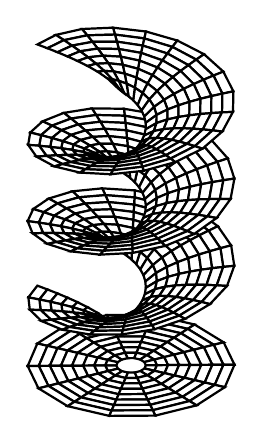
\begin{tikzpicture}[scale=2]
    \begin{axis}[
        axis lines=none,
        axis equal image,
        trig format plots=rad,
        z buffer=sort]
   \addplot3 [
        surf,
        domain=1:7,
        domain y=-pi:pi,
        samples=9,
        samples y=15,
        shader=flat,
        draw=black,
        fill=white
        ]
    ({x*cos(y)},{x*sin(y)},{-12});
   \addplot3 [
        surf,
        domain=1:7,
        samples=9,
        samples y=60,
        shader=flat,
        draw=black,
        fill=white,
        domain y=-3*pi:3*pi
        ]
    ({x*cos(y)},{x*sin(y)},{ln(x)+ y});
    \end{axis}
  \end{tikzpicture}




	      This map \textit{should} be local homeomorphism, but this is false in the Zariski topology. There do not exist nonempty open subsets $V$ and $U$ such that $x \to x^n$ maps $V$ isomorphically onto $U$. The theory of \'etale coverings will give us a good notion of covering which we will use to define the analog of universal coverings
\end{itemize}

The \'etale topology will provide a solution for the problems we have with both cohomology and fundamental groups. The \'etale topology is not a topology in the classical sense, but a category equipped with a notion of covering (in the sense of point-set topology). The analog of open sets of a scheme $X$ will be so called \'etale morphisms $U \to X$. \'Etale morphisms are the natural analogs of local homeomorphisms in scheme theory, so they provide a finer topology than the Zarisiki topology, giving rise to a better sheaf theory. Furthermore, surjective \'etale morphisms share a lot of formal properties with covering spaces, allowing us to define the \'etale fundamental group $\pi_1^{\et}$.
\section{Galois cohomology}
The simplest case of \'etale cohomology is the case of fields. In this case, \'etale cohomology is equivalent to Galois cohomology.
Let $M$ be a $G$ module for $G$ a finite group, meaning that $M$ is an abelian group with a left $G$-action. We will later also consider profinite groups because we are interested in the case of absolute Galois groups. A $G$-module homomorphism is a $G$-equivariant homomorphism. Denote by $M^G = \{m \in M \mid gm = g, \ \forall g \in G\}$ the submodule of $G$-fixed points.
\begin{example}
	Let $G = \Gal(L/k)$. We have the following examples:
	\begin{itemize}
		\item By Galois theory the fixed field of $L$ under $G$ is exactly $L^G = k$
		\item $\mathcal{O}_L^G = \mathcal{O}_k$.
		\item $\mu_n(L)^G = \mu_n(k)$
	\end{itemize}
\end{example}

Let $P, M$, and $N$ be $G$-modules fitting into an exact sequence
\[
	0 \to P \xrightarrow{\alpha} M \xrightarrow{\beta} N \to 0
\]
and let
\[
	P^G \xrightarrow{\alpha'} M^G \xrightarrow{\beta'} N^G
\]
be the resulting sequence. The map $\alpha'$ is just the restriction of an injective map, so $\alpha$ is injective.
Note:
$\ker(\beta') = \ker \beta \cap M^G$

We will show that $im(\alpha') = im(\alpha) \cap M^G$.
Note that $im(\alpha') \subset im(\alpha) \cap M^G$.
For the other inclusion let $m \in im(\alpha) \cap m^G$. There exists a $p \in P$ such that $\alpha(p)=m$. Now let $\sigma \in G,\ \sigma(\alpha(p)) = \sigma(m) = m$,
Since $\alpha(\sigma(p)) = \alpha(p) = m$ and $\alpha$ is injective, $p = \sigma(p)$ so $p$ is fixed under the $G$-action. $im(\alpha) = \ker(\beta) \implies im(\alpha) \cap M^G = \ker(\beta) \cap M^G$.
However, the functor is not right exact:
\begin{example}
	\[1 \to \{\pm 1\} \to \C^\times \to \C^\times \to 1\]
	is exact but
	\[1 \to\{\pm 1\} \to \R^\times \xrightarrow{x \mapsto x^2} \R^\times\]
	is not surjective on the right.
\end{example}

We have shown that the functor $M \to M^G$ is left exact.
% https://math.stackexchange.com/questions/1424102/relationship-between-galois-cohomology-and-etale-cohomology
\[H^1(\Gal(k),M) \cong H_\text{\et}^1(\Spec(k), \widetilde{M})\]

\begin{definition}
	Let $M$ be a $G$-module. The group of $1$-cochains from $G$ to $M$ is defined to be  $C^1(G, M) = \{\varphi: G \to M\}$
\end{definition}

\section{Hilbert's theorem 90}
Let $k$ be a field, $L$ a Galois extension of $k$ and $G = \Gal(L/k)$. A sieve s

